\chapter{Theoretical Introduction}
\section{Background}

In the current digital landscape, cyber incidents can have severe consequences of which evidence suggests can have been mitigated through appropriate safeguards. As modern societies increasingly depend on digital infrastructure, cyber risk management has become essential. Approximately 65 \% of the world's population is online \citep{hanji_machine_2023}, and global e-commerce accounts for roughly one-third of world GDP \citep{wysokinska_global_2023}, meaning that a substantial share of economic and social activity now occurs in cyberspace. This rise in digital connectivity has created a larger attack surface, with research indicating that increased internet usage and digitization are associated with higher levels of cybercrime and greater opportunities for exploitation \citep{figueiredo_alves_silva_digital_2024}. At the same time, the consequences of cyber incidents can be substantial, for example, the global average cost of a single data breach was estimated at about USD 4.45 million in 2023. Given that risk management frameworks reduce incident likelihood \citep{jung_effect_2025}, paired with growing exposure and the significant potential impact of cyber incidents, the need for effective cyber risk management becomes evident.

One example of such a cyber risk management methodology is CORAS, a model-driven risk analysis method that provides a structured process supported by a visual modelling language \citep{kpoze_cybersecurity_2023}. The methodology follows a step-wise workflow and includes tool support and UML-based modelling, visually representing threats, vulnerabilities, and risks \citep{kpoze_cybersecurity_2023}. Empirical studies have shown that CORAS is generally perceived as more usable than several alternative security risk assessment methods\footnote{Empirical comparisons have evaluated CORAS against other security requirements and risk analysis methods, including Secure Tropos, Secure i*, and Problem Frames, and found CORAS to be substantially more usable for participants in controlled experiments \citep{broccia_evaluating_2025}.}, and that visual modelling approaches can improve understanding and communication during risk analysis \citep{broccia_evaluating_2025}. CORAS has been applied in various domains such as maritime cybersecurity case studies and in critical infrastructures such as power-grid systems, demonstrating the methodology's applicability for cyber risk management \citep{kpoze_cybersecurity_2023,erbas_systematic_2024}.

\section{CORAS seven step analysis}
As previously mentioned, CORAS is a stepwise methodology. Early presentations of the CORAS method describe the analysis process in seven main steps \citep{braber_model-based_2007}, whereas later and more detailed descriptions present it as an eight-step process \citep{lund_model-driven_2011}. In this report we adopt the simplified seven-step presentation. These seven steps can be mapped to the overall 5 step risk management process where the first three CORAS steps maps to the first process, and the following steps maps one-to-one with the corresponding processes. Figure~\ref{fig:coras_mapping} shows how the seven-step CORAS presentation maps to the general five-step risk management process, where CORAS refines the context-identification process into several introductory activities.

\begin{figure}[htbp]
  \centering
  \resizebox{0.85\textwidth}{!}{
    
\begin{tikzpicture}[
    font=\small,
    processL/.style={
      rectangle,
      draw=dtured,
      fill=dtured,
      text=white,
      font=\bfseries,
      line width=0.8pt,
      minimum width=5.0cm,
      minimum height=0.95cm,
      text width=4.3cm,
      align=left,
      inner xsep=10pt,
      inner ysep=6pt
    },
    processR/.style={
      rectangle,
      draw=blue,
      fill=blue,
      text=white,
      font=\bfseries,
      line width=0.8pt,
      minimum width=5.0cm,
      minimum height=0.95cm,
      text width=4.3cm,
      align=left,
      inner xsep=10pt,
      inner ysep=6pt
    },
    mapbox/.style={
      rectangle,
      draw=black!45,
      fill=grey!20,
      text=black,
      line width=0.8pt,
      minimum width=2.8cm,
      minimum height=0.95cm,
      text width=2.2cm,
      align=center,
      inner xsep=6pt,
      inner ysep=4pt
    },
    heading/.style={
      font=\bfseries\small,
      text=black,
      align=center
    },
    line/.style={
      draw=black!70,
      line width=1.0pt
    }
  ]

  % headings
  \node[heading] at (0,5.15) {General risk management\\process};
  \node[heading] at (8.2,5.15) {CORAS 7-step\\presentation};

  % left column
  \node[processL] (g1) at (0,4.1)  {1. Identify context};
  \node[processL] (g2) at (0,2.8)  {2. Identify risks};
  \node[processL] (g3) at (0,1.5)  {3. Analyse risk};
  \node[processL] (g4) at (0,0.2)  {4. Risk evaluation};
  \node[processL] (g5) at (0,-1.1) {5. Risk treatment};

  % right column
  \node[processR] (c1) at (8.2,4.7)  {1. Introduction};
  \node[processR] (c2) at (8.2,3.7)  {2. High-level analysis};
  \node[processR] (c3) at (8.2,2.7)  {3. Approval};
  \node[processR] (c4) at (8.2,1.5)  {4. Risk identification};
  \node[processR] (c5) at (8.2,0.3)  {5. Risk estimation};
  \node[processR] (c6) at (8.2,-0.9) {6. Risk evaluation};
  \node[processR] (c7) at (8.2,-2.1) {7. Risk treatment};

  % straight lines only
  \draw[line] (g1.east) -- (c1.west);
  \draw[line] (g1.east) -- (c2.west);
  \draw[line] (g1.east) -- (c3.west);
  \draw[line] (g2.east) -- (c4.west);
  \draw[line] (g3.east) -- (c5.west);
  \draw[line] (g4.east) -- (c6.west);
  \draw[line] (g5.east) -- (c7.west);

  % grouping on right
  \draw[black!45, line width=0.8pt] (10.95,5.0) -- (11.1,5.0);
  \draw[black!45, line width=0.8pt] (11.1,5.0) -- (11.1,2.4);
  \draw[black!45, line width=0.8pt] (10.95,2.4) -- (11.1,2.4);

  \node[
    text=black,
    line width=0.8pt,
    minimum height=0.9cm,
    text width=2.4cm,
    align=center
  ] at (12.75,3.7) {Introductory\\activities};

\end{tikzpicture}%

  }
  \caption{Mapping between the general five-step risk management process and the seven-step CORAS method.}
  \label{fig:coras_mapping}
\end{figure}

\subsection{Step 1: Introduction}
In the first step, the scope and focus of the analysis are established so that the analysts and stakeholders share a common understanding of the system under consideration and the assets that need protection. This step typically involves a meeting between the analysts and the stakeholders. The analysts introduce the CORAS method and the purpose of the analysis, after which the stakeholders present the target system to be analysed. The meeting concludes with a discussion to clarify the analysis context and expectations. By the end of Step 1, the following aspects should be agreed upon:

\begin{itemize}
  \item Analysis focus and scope
  \item Informal description of the target system and its assets
  \item Relevant background documentation (e.g., regulations, contracts, guidelines)
  \item Common terminology and methods
  \item Assumptions
  \item Roles and responsibilities
  \item A plan for the analysis, including dates for meetings and delivery of reports
\end{itemize}

\subsection{Step 2: High Level Analysis}
In a second meeting the analysits presents their understanding of the targets static and dynamic feauters and invites the customer to correct their understanding where needed. This can be done by the analysts presenting UML diagrams, for example, class diagram illustrating the overview of the target; collaboration diagrams showing the entities in the target such as network, sites, or hardware; and activity or sequence diagrams illustrating processes and data-flows.

\begin{figure}[htbp]
  \centering
  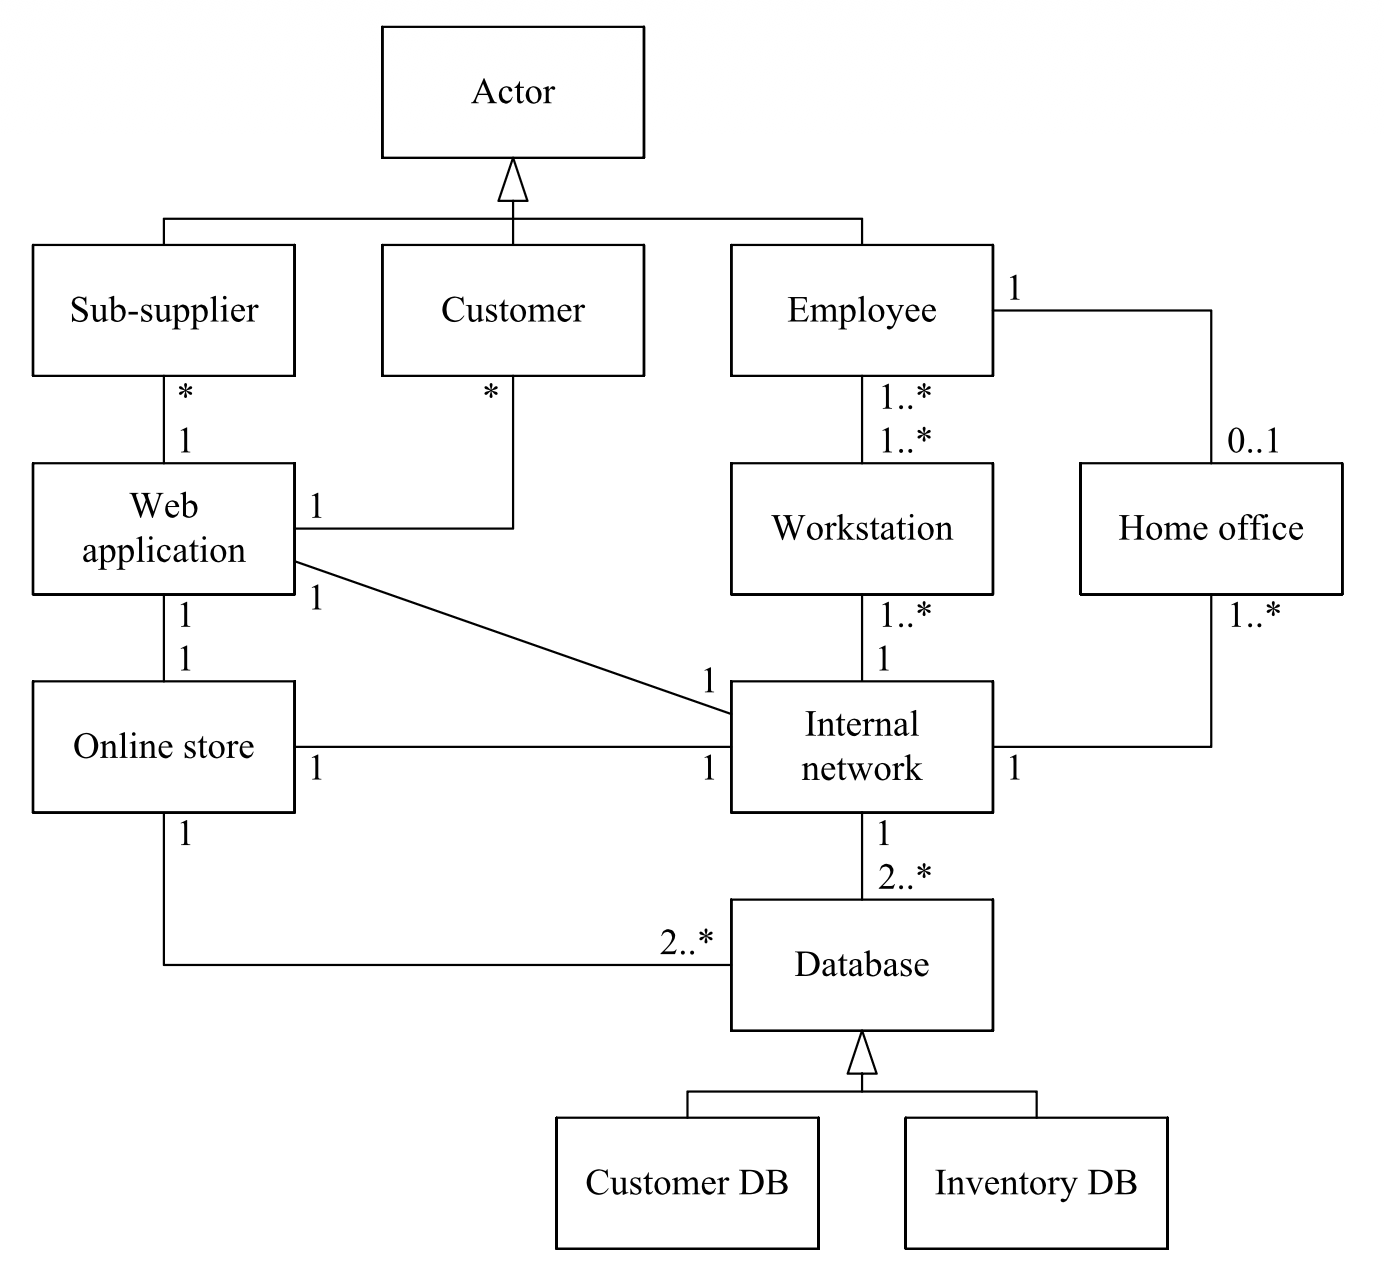
\includegraphics[width=0.8\textwidth]{figures/uml_class_diagram_target.png}
  \caption{}
  \label{fig:target_class_diagram}
\end{figure}

The analysts then presents a CORAS asset diagrams of the assets they have identified. Through discussion between the analysts and the customer the assets diagram is refined and threats, vulnerabilities, threat scenarios, and unwanted incidents are identified and documented as \textit{target descriptions} in a high level risk analysis table. Finally the most important related threats and vulnerabilities are brainstormed.

\subsection{Step 3: Approval}
"The analysts team presents the documentation of the target of analysis for finalisation and approval by the customer; values are assigned to the identified assets, and the risk evaluation criteria are established"

\subsection{Step 4: Risk identification}
"Risks are identified through a structured brainstorming"

\subsection{Step 5: Risk estimation}
"The likelihoods and consequences for the identified risks are estimated"

\subsection{Step 6: Risk evaluation}
"The risks are evaluated against the risk evaluation criteria"

\subsection{Step 7: Risk treatment}
"Treatments for the mitigation of unacceptable risks are identified and evaluated"
